% vim:encoding=utf8 ft=tex sts=2 sw=2 et:

\documentclass{classrep}
\usepackage[utf8]{inputenc}
\usepackage{fixltx2e}
\usepackage{url}
\usepackage{graphicx}
\usepackage{siunitx}


\studycycle{Informatyka, studia niestacjonarne, inż I st.}
\coursesemester{VI}

%\coursename{hhhhhhhheoretyczna i stosowana}
\coursename{Inteligentna Analiza Danych}
\courseyear{2013/2014}

\courseteacher{mgr inż. Michał Pryczek}
\coursegroup{sobota, 11:15}

\author{
  \studentinfo{Łukasz Ochmański}{183566} \and
  \studentinfo{Przemysław Szwajkowski}{173524}
}

\title{Zadanie 2b: Perceptron Wielowarstwowy}
\svnurl{http://iad-lukasz-ochmanski.googlecode.com/svn/trunk/02}

\begin{document}
\maketitle


\section{Cel}
Dokonać redukcji/transformacji wybranych w części pierwszej cech dla rozważanych zbiorów danych (należy również rozważyć zbiór Iris Flower Data Set). Redukcji/transformacji należy dokonać na dwa sposoby:
\\
    Poprzez odrzucenie części cech.
    Poprzez wykorzystanie wyjść z warstwy ukrytej sieci MLP trenowanej w trybie autoasocjacji.
\\
Stworzona aplikacja powinna umożliwiać maksymalną elastyczność pod względem możliwości wyboru sposobu redukcji/transformacji cech (w sprawozdaniu dla każdego zbioru wystarczy w obu przypadkach przeprowadzić eksperymenty dla dwóch zredukowanych/przetransformowanych zestawów cech, z których jeden będzie dwuelementowy).
\\
Należy zwrócić uwagę na następujące elementy:
\begin{itemize}
	\item Sposób wyboru zbiorów: treningowego, testowego i walidacyjnego.
  \item Zdolności uogólniające sieci i zjawisko przeuczenia.
  \item Zgodność wniosków z analizy rozważanych zbiorów wykonanej  w zadaniu 1 z uzyskanymi wyniami w tym zadaniu.
\end{itemize}

\section{Wstęp}
W badaniu uwzględniono poniższe konfiguracje sieci perceptronowej:
\begin{itemize}
\item
1. 4-2-3
\item
2. 3-2-3
\item
3. 3-2-2
\item
4. 3-2-3
\item
5. 3-2-3
\item
6. 2-2-3
\item
7. 2-2-2
\item
8. 2-2-3
\item
9. 2-2-3
\end{itemize}

\\*

\begin{figure}[ht]
\centering
			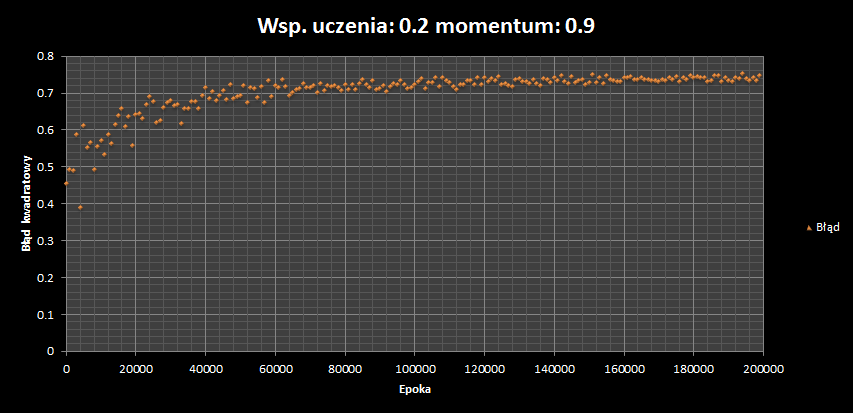
\includegraphics[scale=0.65]{pictures/Iris01.png}
	\caption{Iris data set}
	\label{fig:Iris data set}
\end{figure}

\begin{figure}[ht]
\centering
			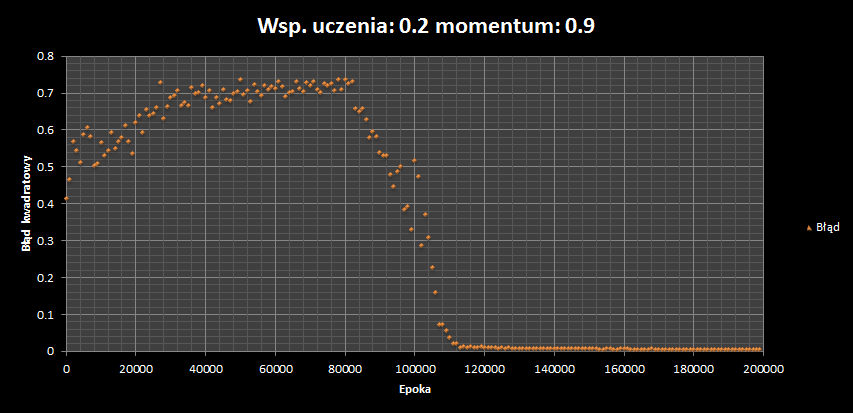
\includegraphics[scale=0.65]{pictures/Iris02.png}
	\caption{Iris data set}
	\label{fig:Iris data set}
\end{figure}

\begin{figure}[ht]
\centering
			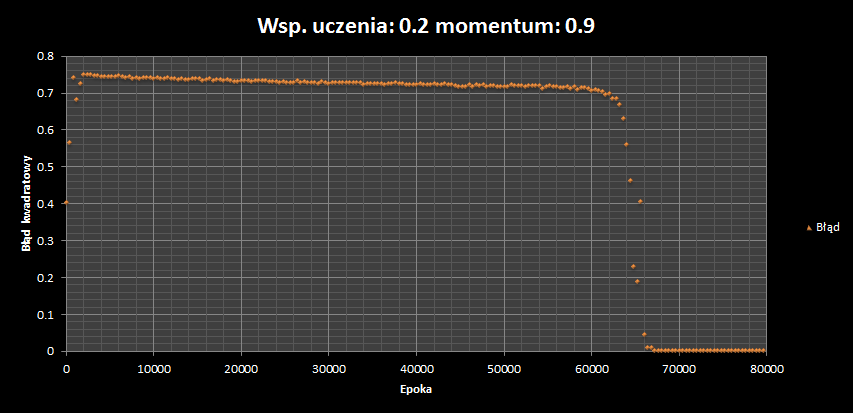
\includegraphics[scale=0.65]{pictures/Iris03.png}
	\caption{Iris data set}
	\label{fig:Iris data set}
\end{figure}

\begin{figure}[ht]
\centering
			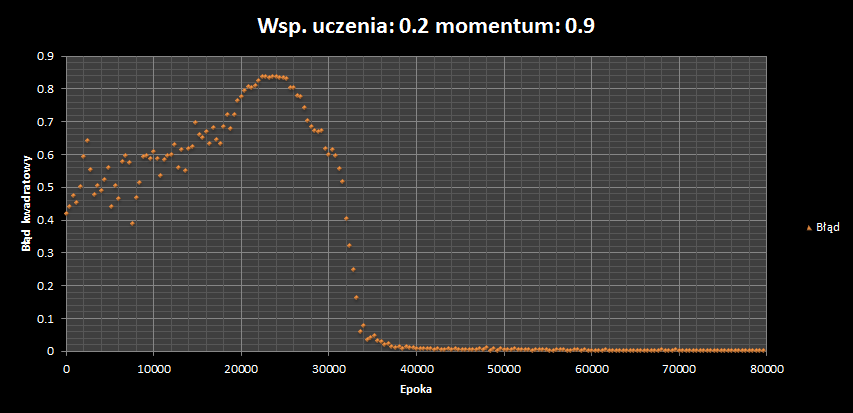
\includegraphics[scale=0.65]{pictures/Iris04.png}
	\caption{Iris data set}
	\label{fig:Iris data set}
\end{figure}

\begin{figure}[ht]
\centering
			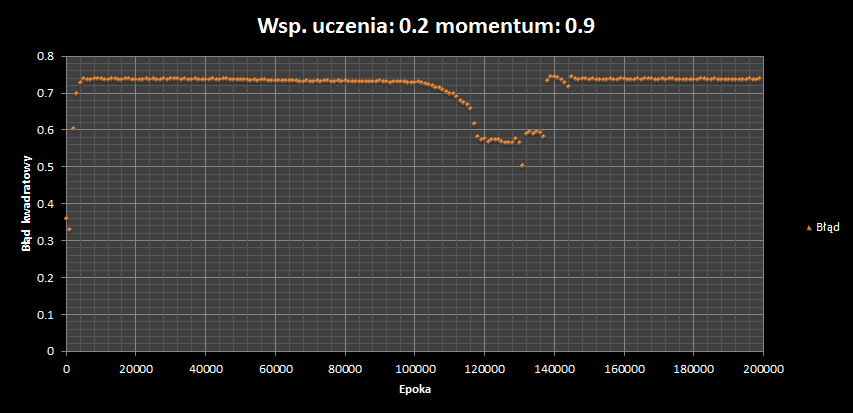
\includegraphics[scale=0.65]{pictures/Iris05.png}
	\caption{Iris data set}
	\label{fig:Iris data set}
\end{figure}

\begin{figure}[ht]
\centering
			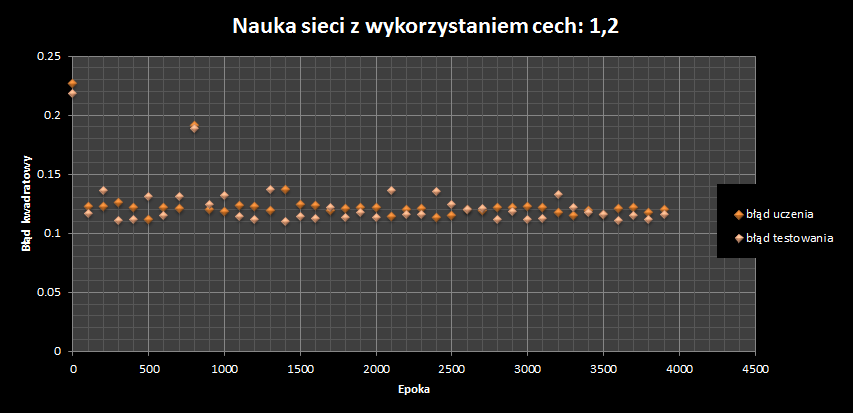
\includegraphics[scale=0.65]{pictures/Iris06.png}
	\caption{Iris data set}
	\label{fig:Iris data set}
\end{figure}

\begin{figure}[ht]
\centering
			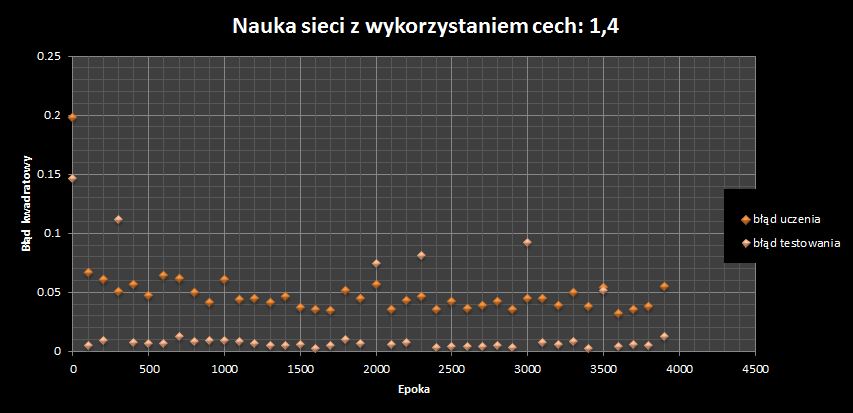
\includegraphics[scale=0.65]{pictures/Iris07.png}
	\caption{Iris data set}
	\label{fig:Iris data set}
\end{figure}

\begin{figure}[ht]
\centering
			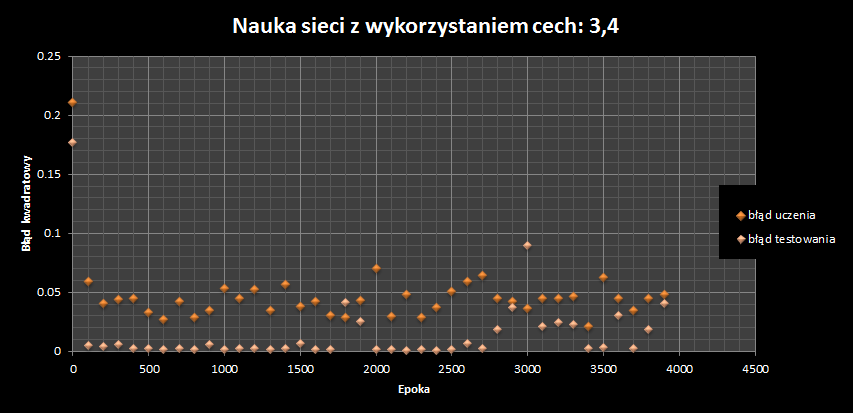
\includegraphics[scale=0.65]{pictures/Iris08.png}
	\caption{Iris data set}
	\label{fig:Iris data set}
\end{figure}

\begin{figure}[ht]
\centering
			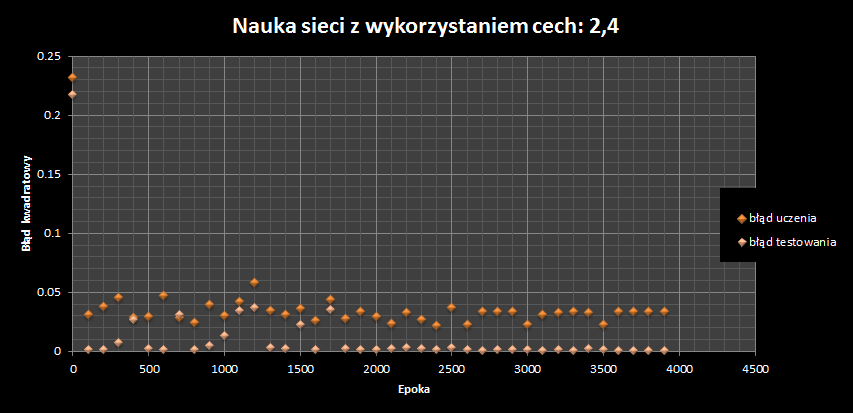
\includegraphics[scale=0.65]{pictures/Iris09.png}
	\caption{Iris data set}
	\label{fig:Iris data set}
\end{figure}

\clearpage

Badania zostały przeprowadzone na zbiorze treningowym oraz na zbiorze testowym, w którym zbiór treningowy składa się ze 135 elementów, a zbiór testowy z 15 elementów. Wszystkich elementów było 150. Zbiór treningowy i zbiór testowy były rozłączne. Celem takiego podziału jest uniknięcie sytuacji, w której sieć nauczy się rozpoznawać tylko przedstawione wcześniej wzorce. Chcemy, aby sieć posiadała ogólną więdzę i potrafiła rozpoznać nawet wzorce wcześniej niespotykane. Taką właściwość nazywamy zdolnością generalizacyjną sieci neuronowej.

\begin{figure}[ht]
\centering
			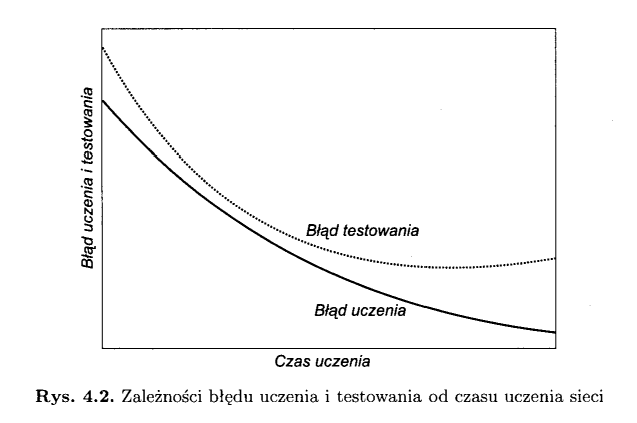
\includegraphics[scale=0.65]{pictures/Iris11.png}
	\caption{Iris data set}
	\label{fig:Iris data set}
\end{figure}

Pomimo usilnych prób nie udało się osiągnąć oczekiwanych rezultatów. Jak widać na powyższym ryskunku wraz z upływem czasu błąd uczenia powinien maleć, a błąd testowania powinien albo pozostać stały, bądź zacząć rosnąć pomimo, że błąd nauki maleje. Z wykresu na rysunku wynika jednoznacznie, że zbyt długie uczenie może doprowadzić do tzw. przeuczenia sieci.

\begin{figure}[ht]
\centering
			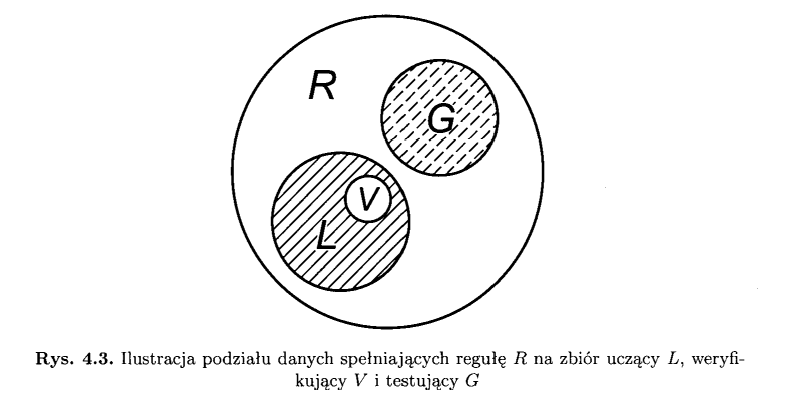
\includegraphics[scale=0.65]{pictures/Iris10.png}
	\caption{Iris data set}
	\label{fig:Iris data set}
\end{figure}

W celu uniknięcia przeuczenia wydziela się ze zbioru uczącego częśc danych weryfikujących (zbiór V na ryskunku 4.3), które służą w procesie uczenia okresowemu sprawdzaniu aktualnie nabytych zdolności generalizacyjnych. Gdy błąd generalizacji zaczyna się zwiększać, należy przerwać naukę.


\clearpage

\begin{thebibliography}{0}
  \bibitem{l2short} \textsl{Stanisław Osowski} - Sieci neuronowe do przetwarzania informacji, \textsl{Wyd. 2., Warszawa 2006}
  \bibitem{l2short} ``Learning and neural networks'' [\url{http://en.wikiversity.org/wiki/Learning_and_neural_networks}]
  \bibitem{l2short} UCI Machine Learning Repository \textsl{Iris Data Set}
\end{thebibliography}
\end{document}